\section{Implementation}
\label{sec-impl}

In \S \ref{sec-methods} the strategies and interfaces that \Cyclus uses to 
simplify archetype development were presented. These represent notions about
the amount of information and prior knowledge that the archetype developer 
must have in order to write archetypes.  If a particular particular strategy 
decreased the knowledge required by archetype developers then it is considered
easier and beneficial to implement.  

However, methods that are more inuitive for new users to understand are often
propotionatly more difficult to implement. For example, it is one thing to 
learn to play the game \emph{tic-tac-toe}, or even master it; it is quite another
thing to design the game \emph{tic-tac-toe} in the first place.  
A sublime interface belies 
herculean effort. This section descibes the infrastructre that holds up 
current \cyclus archetype development.  This is relevant to other fuel 
cycle simulators that wish to adopt the same strategies that \cyclus 
implements. In particular, the implemention of the \cyclus preprocessor, 
the type system, input file validation, metadata annotations will all 
be covered here.

\subsection{The \Cyclus Preprocessor}

The \cyclus preprocessor, \cycpp, is resposnible for all metadata collection and 
code generation for archetypes. It is implemented as a small Python utility 
currently less than 2000 lines in a single file.  It has no dependencies other 
than the Python standard library. It is thus light-weight enough to move around 
between code projects, if needed. For the scale of its responsibility, \cycpp
is extremely efficient. 

The preprocessor implements the three passes detailed in \S\ref{subsec-ppgc}:
normalization via standard \code{cpp}, state variable annotation accumulation, and code 
generation. The \cycpp tool must be run on all C++ header and source files that
contain archetype code and the \code{#pragma cyclus} directives. Running \cycpp
on files without such directives does no harm and will result in exactly the 
original file. The first \cycpp
pass, running the C preprocessor over these files, is a trivial subprocess 
spawn. The only potential trouble spots here are ensureing that \cycpp sees the
same include, macro defintitions, and macro undefinitions that actual compilation 
of the source code will have.

The second pass, state accumulation, represents half of the work that \cycpp performs.
The results from pass 1 is fed into this pass and scoured for 
potentially relevant information about the archetypes present in the file. 
Thus, state accumulation 
may be thought of as a traditional parser which tranforms tokens (line of the 
C++ file) into a more meaningful in-memory data structure. As a parser, pass 2 
may be implemented as a \emph{state machine} \cite{mertz2003text,wagner2006modeling}.

Pass is represented in \cycpp by the \code{StateAccumulator} class.  This is a
state machine which takes lines output from the C preproessor and compares them 
against a seires of \emph{filters}.  If a line matches the expected structure 
for a filter, then the filter executes a \emph{transformation} function on the 
line and no further filters are executed. If the line does not match any filters
then the line is allowed to pass through the \code{StateAccumulator}. 
The filter-transformation sequence can be thought of in analogy to a sphere of a 
given radius (a line of code) attempting to pass through concentric windows 
(the filters) of decreasing appeture. This first windown where the sphere stops 
represents the transformation that is executed.  This sphere is allowed to 
move through the system without being stopped. This analogy may be seen in 
Figure \ref{filter-analogy}.

\begin{figure}[htbc]
\label{filter-analogy}
\centering
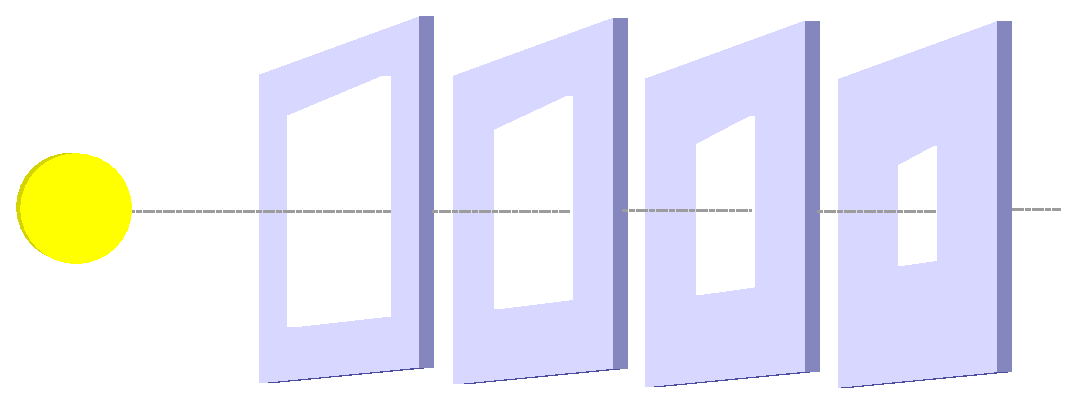
\includegraphics[width=0.8\textwidth]{filter-analogy.eps}
\caption{The \code{StateAccumulator} class passes lines of C++ code through 
a series of filters, each of which may transform the information heretofore gathered
by previous filters. 
This may be thought of analogous to a spheres of various radii rolling through 
concentric windows.  The spheres, or lines, stop rolling when they hit a  
window, or filter. This triggers the execution of the transformation function of just 
that filter and that filter alone.}
\end{figure}


\subsection{Database Types \& Backends}

\textbf{Robert C. and Anthony}

\subsubsection{Hashability}

\subsection{XML Validation}

\textbf{Katy}

\subsection{JSON Annotations}

\textbf{Radio}
